\section{OT-Security}

\subsection{Abgrenzung IT-Security und OT-Security}

Die Unterscheidung zwischen IT-Security und OT-Security ist in der Sicherheitsarchitektur industrieller Systeme von zentraler Bedeutung. Während IT-Security hauptsächlich darauf abzielt, Informations- und Kommunikationstechnologien zu sichern, konzentriert sich OT-Security auf die Absicherung von Steuerungs- und Automatisierungstechnologien, die direkt physikalische Prozesse in industriellen Umgebungen beeinflussen. Mit OT meint es "[...] Hard- und Software, die physische Geräte, Prozesse und Ereignisse in der Institution überwacht und steuert" (\cite {ICS}, S. 9). Diese Unterschiede zeigen sich auch in der grundlegenden Denkweise: Während die IT virtuell ist, ist die OT physisch. Ein weiterer wesentlicher Unterschied liegt in den Schutzzielen, die unterschiedlich priorisiert werden. Gemäß des BSI sind die primären Schutzziele wie folgt definiert (vgl. \cite{BSI}): 
\begin{itemize}
\item \textbf{Vertraulichkeit}: Nur autorisierte Personen haben Zugriff zu den Informationen.
\item \textbf{Integrität}: Die Information wurde auf dem Transportweg nicht verändert.
\item \textbf{Verfügbarkeit}: Kommunikationsdienste stehen zu den gewünschten Zeitpunkten zur Verfügung.
\end{itemize}
Zusätzlich zu diesen Zielen spielt in der OT-Security auch das Schutzziel Safety eine bedeutende Rolle. Safety zielt darauf ab, Personen und die Umwelt vor physischen Schäden zu schützen, indem Maßnahmen ergriffen werden, um Unfälle zu verhindern oder ihre Auswirkungen zu minimieren (vgl. \cite{Safety}). Die unterschiedliche Hierarchie der Schutzziele wird in den folgenden Abbildungen veranschaulicht:
\begin{figure}[h]
    \centering
    \begin{minipage}{0.45\textwidth}
        \centering
        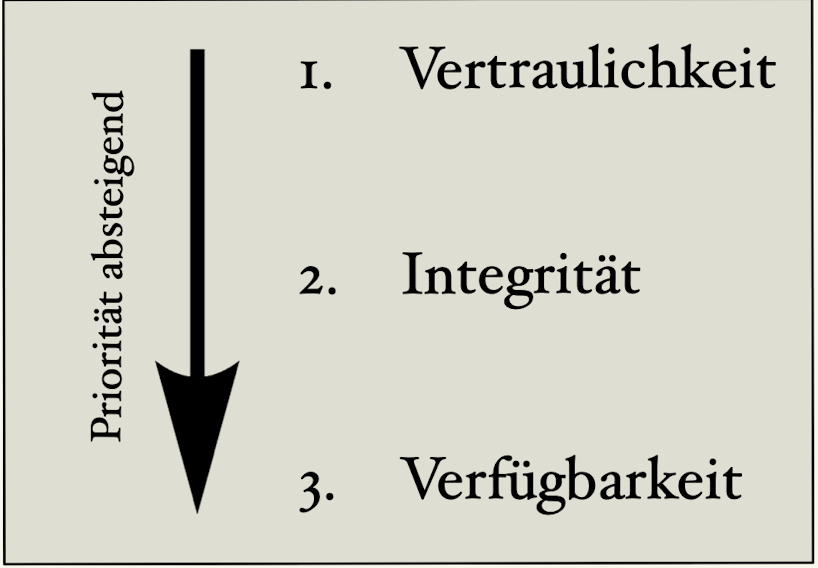
\includegraphics[scale=.3]{images/ITS.png}
        \caption{Schutzziele IT-Security}
        \label{fig:meine-grafik1}
    \end{minipage}
    \hfill
    \begin{minipage}{0.45\textwidth}
        \centering
        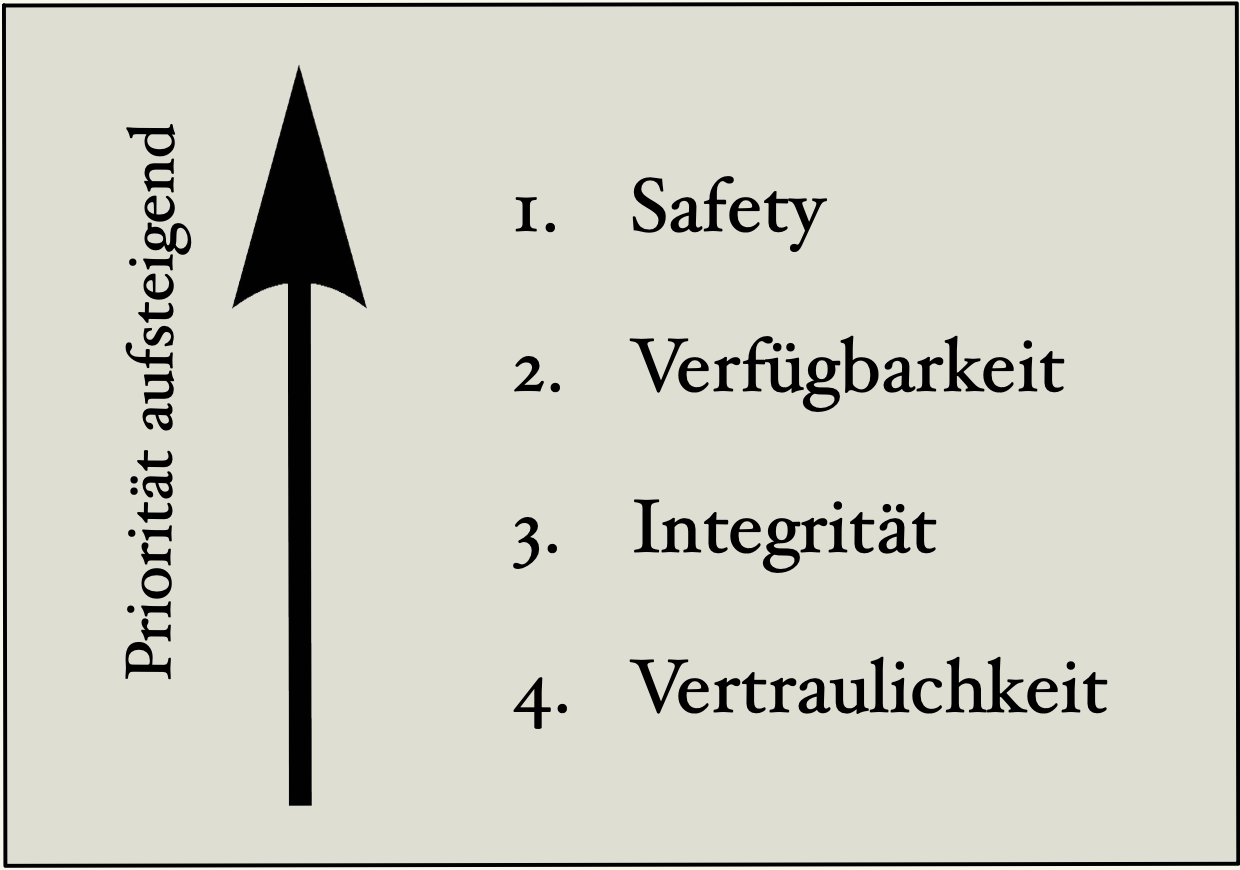
\includegraphics[scale=.299]{images/OTS.png}
        \caption{Schutzziele OT-Security}
        \label{fig:meine-grafik2}
    \end{minipage}
\end{figure}
\\ Konzeptionell verfolgen beide Ansätze verschiedene Rangordnungen der Schutzziele. Für die OT-Security ist die Verfügbarkeit industrieller Anlagen zu jedem Zeitpunkt von besonderer Bedeutung. Für Industriebetriebe ist dies essenziell, da ungeplante Ausfallzeiten im Schnitt 532.000 US-Dollar pro Stunde kosten (vgl. \cite{OTS/ITS}). 
\subsection{Herausforderungen und Bedrohungslage}

Das ICS Security Kompendium des BSI ist ein Grundlagenwerk, das Organisationen dabei unterstützt, Cybersicherheitsrisiken in der OT zu erkennen und zu bewältigen, indem es Basiswissen vermittelt, Maßnahmen und Prozesse beschreibt sowie Verbindungen zu relevanten Standards und Gesetzen herstellt. Hierbei werden drei grundsätzliche Schwachstellen im OT-Umfeld definiert. Man unterteilt in Organisatorische Schwachstellen, Technische Schwachstellen und die Schwachstelle Lieferkette. 

\subsubsection{Organisatorische Schwachstellen}

Die Sicherheit industrieller Steuerungssysteme (OT-Umgebungen) ist essenziell für die Aufrechterhaltung kritischer Infrastrukturen, aber oft durch diverse organisatorische Schwachstellen gefährdet. Eine zentrale Schwäche liegt in unzureichenden oder fehlenden organisatorischen Regelungen sowie einer mangelhaften Dokumentation zur Cybersicherheit. Diese bilden die Grundlage für effektive Entscheidungsfindung und Maßnahmen, und ihr Fehlen kann potenzielle Sicherheitslücken verursachen, die ausgenutzt werden könnten.
Ein weiteres kritisches Problem ist das unzureichende Risikomanagement in OT-Umgebungen. Ohne eine gründliche Identifikation und Bewertung potenzieller Gefahren können Schwachstellen und Bedrohungen übersehen oder falsch priorisiert werden, was zu ungeeigneten oder unzureichenden Schutzmaßnahmen führt. Dies wiederum könnte die Reaktionsfähigkeit auf Sicherheitsvorfälle beeinträchtigen und die Auswirkungen solcher Zwischenfälle verschlimmern. Ein bedeutender Aspekt ist auch die mangelnde Kommunikation innerhalb der Organisationen. Klar definierte Richtlinien und Verfahren müssen nicht nur vorhanden sein, sondern auch effektiv kommuniziert werden, um Missverständnisse zu vermeiden und sicherzustellen, dass Sicherheitsmaßnahmen korrekt umgesetzt werden. Eine unzureichende Dokumentation und Kommunikation können im Ernstfall zu erheblichen Verzögerungen bei der Fehlerdiagnose und -behebung führen, was die Ausfallzeiten und die Wiederherstellungszeiten erhöht. Ein weiteres Problem ergibt sich aus der Übertragung ungeeigneter IT-Praktiken auf das OT-Umfeld. Da IT- und OT-Systeme unterschiedliche Anforderungen und Betriebsabläufe haben, können Sicherheitsmaßnahmen und -standards aus der IT nicht einfach auf OT-Systeme übertragen werden. Dies kann zu inkonsistenten oder unzureichenden Sicherheitslösungen führen, die die spezifischen Risiken und Bedrohungen in OT-Umgebungen nicht angemessen berücksichtigen (vgl. \cite{ICS}, S. 31-34).

\subsubsection{Technische Schwachstellen}

In der Analyse der technischen Schwachstellen von OT-Systemen zeigt sich eine Vielzahl von Risiken, die durch unzureichende Sicherheitsmaßnahmen und veraltete Konfigurationen entstehen können. Ein zentraler Aspekt ist die unvollständige Absicherung von Fernzugängen, die autorisierten Personen ermöglichen, aus der Ferne auf Systeme zuzugreifen. Besonders relevant ist dies im Kontext zunehmender Nutzung von Homeoffice und mobilen Zugängen, jedoch sind diese Zugänge oft schlecht geschützt und können Angriffspunkte für Cyberkriminelle darstellen. Ein weiteres bedeutendes Risiko ergibt sich aus der fehlenden Überwachung der Infrastruktur, die dazu führen kann, dass sicherheitsrelevante Ereignisse und Schwachstellen nicht rechtzeitig erkannt werden. Dies birgt die Gefahr von Produktionsausfällen und Sicherheitsvorfällen, die erhebliche wirtschaftliche Schäden verursachen können. Zusätzlich sind OT-Netze zunehmend von IT-Netzen abhängig, was potenzielle Sicherheitslücken durch gemeinsam genutzte Infrastruktur und Dienste schafft. Störungen oder Angriffe in IT-Netzen können sich direkt auf OT-Umgebungen auswirken und zu schwerwiegenden Konsequenzen führen, wie z.B. Produktionsausfällen oder sogar Sicherheitsrisiken für Mensch und Umwelt. Ein weiteres kritisches Thema ist die Verwendung von Legacy-Systemen, die aufgrund ihrer veralteten Sicherheitsmechanismen und der fehlenden Herstellerunterstützung besonders anfällig für Cyberangriffe sind. Diese Systeme können moderne Sicherheitsbedrohungen oft nicht effektiv abwehren und stellen somit ein erhebliches Risiko für die Sicherheit von OT-Umgebungen dar (vgl. \cite{ICS}, S. 34-39). 


\subsubsection{Schwachstelle Lieferkette}

Die Lieferketten für industrielle Steuerungssysteme haben in den letzten Jahren verstärkt das Interesse von Cyberangreifern auf sich gezogen. Diese Angreifer nutzen gezielt Schwachstellen in der Lieferkette aus, um Schadsoftware oder Hintertüren in die OT-Komponenten einzuschleusen. Dadurch können sie unautorisierten Zugriff auf kritische Infrastrukturen wie Stromnetze, Wasserversorgung oder Verkehrssteuerungssysteme erlangen.
Ein zentraler Aspekt sind unzureichende Sicherheitsregelungen innerhalb der Lieferkette. Wenn die Verantwortlichkeiten für die Cybersicherheit nicht klar geregelt sind, entstehen Gefahrenpunkte, da niemand sich zuständig fühlt, potenzielle Schwachstellen zu identifizieren und zu beheben. Hardware-Hintertüren sind eine weitere schwerwiegende Schwachstelle. Diese ermöglichen es Herstellern oder Dritten, verdeckte Zugänge zu Systemen oder Daten einzurichten. Solche Hintertüren können durch das Hinzufügen von Schnittstellen oder speziellen Codes in die Firmware oder das BIOS der OT-Komponenten entstehen. Die Firmware, als entscheidendes Element für die Funktion der Steuergeräte, ist ebenfalls anfällig für Schwachstellen. Diese können durch fest einprogrammierte Zugangsdaten oder fehlerhafte Entwicklungspraktiken entstehen. Modifizierte Firmware, die während des Transports oder durch kompromittierte Updates eingespielt wird, ermöglicht es Angreifern, Geräte fernzusteuern oder sensible Daten auszulesen. Die Kryptographie, die zur Sicherung von Daten verwendet wird, ist nicht immun gegen Schwachstellen. Fehlerhafte Implementierungen oder veraltete Verfahren können es Angreifern erleichtern, verschlüsselte Daten zu entschlüsseln oder Manipulationen vorzunehmen. Neben der Firmware sind auch Anwendungssoftware und deren Integration in die IT-Infrastruktur potenzielle Einfallstore für Angreifer. Standard IT-Betriebssysteme wie Windows oder Linux, die für diese Anwendungen genutzt werden, sind selbst häufig Ziel von Cyberangriffen. Ein unsicherer Beschaffungsprozess, bei dem Cybersicherheitsanforderungen nicht ausreichend berücksichtigt werden, trägt ebenfalls zur Verwundbarkeit der Lieferkette bei. Ebenso können Fehler bei der Implementierung und Integration von Anlagenkomponenten durch verschiedene Hersteller Sicherheitslücken erzeugen, die ausgenutzt werden können. Externe Dienstleister, die unsichere Geräte oder ungeprüfte Zugriffe auf Anlagen verwenden, stellen ein weiteres Risiko dar. Ebenso birgt die Nutzung externer Plattformen und Cloud-Infrastrukturen Herausforderungen wie mangelnde Kontrolle über Sicherheitsmaßnahmen und potenzielle Schwachstellen bei der Datenübertragung (vgl. \cite{ICS}, S. 39-41).

\subsection{Maßnahmen}


Im Bereich der OT-Security sind gezielte Maßnahmen entscheidend, um die Sicherheit industrieller Steuerungssysteme zu gewährleisten. ,,OT-Sicherheit hat bisher keine Priorität in Deutschland'' (\cite{CISCO}), so der „State of Industrial Networking Report“ von CISCO, einem weltweit führenden Unternehmen im Bereich Netzwerktechnologie. Angreifer nutzen zunehmend fortschrittliche Werkzeuge, einschließlich Künstlicher Intelligenz, um ihre Angriffe zu verfeinern, weshalb ein kontinuierliches Update der Sicherheitstechnologien und -praktiken unerlässlich ist. Die Übertragung von IT-Sicherheitsmaßnahmen auf OT-Umgebungen ist jedoch komplex, da nicht alle Maßnahmen problemlos anwendbar sind. Beispielsweise können Schadsoftware-Scanner in Produktionsumgebungen zu Ausfällen führen, was dem Schutzziel der Verfügbarkeit widerspricht.

Die Segmentierung von Netzwerken stellt eine bewährte Strategie dar, um die Netzwerksicherheit zu verbessern. Dieser Ansatz teilt ein größeres Netzwerk in kleinere, autonome Subnetze auf, was eine bessere Überwachung, Kontrolle des Datenverkehrs sowie eine optimierte Netzwerkleistung ermöglicht. Zudem erleichtert er die Identifikation und Behebung technischer Probleme und schränkt die Ausbreitung von Malware innerhalb des Netzwerks ein (vgl. \cite{Netzwerksegmentierung}).

Die Netzwerkzugangskontrolle (Network Access Control, NAC) regelt, wer Zugriff auf das Netzwerk erhält und in welchem Umfang. Dies geschieht durch Authentifizierung, Identifizierung von Benutzern und Geräten sowie entsprechende Zuordnung und Autorisierung der Kommunikationsverbindungen. Während NAC-Systeme in der IT weit verbreitet und einfach zu implementieren sind, stellen sie in der Operational Technology (OT) spezifische und komplexere Anforderungen dar. Eine fehlerhafte Zuordnung oder Abkopplung eines Geräts in der OT kann erhebliche Auswirkungen auf die Anlagenverfügbarkeit haben (vgl. \cite{NAC}).

Der Einsatz von künstlicher Intelligenz (KI) gewinnt zunehmend an Bedeutung in der Sicherheitsbranche, da er sowohl neue Angriffsmöglichkeiten eröffnet als auch fortschrittliche Abwehrstrategien ermöglicht. KI-Technologien bieten den entscheidenden Vorteil, dass sie Bedrohungen und Anomalien erheblich schneller und präziser erkennen können als Menschen. Diese Systeme entwickeln sich kontinuierlich weiter und passen sich dynamisch an neue Gefahren an, was in einer sich ständig verändernden Sicherheitslandschaft unverzichtbar ist. Durch Anomalieerkennung, Verhaltensanalyse und prädiktive Methoden kann KI potenzielle Gefahren frühzeitig identifizieren, indem sie ungewöhnliche Muster und Verhaltensweisen im System aufspürt (vgl. \cite{hornetsec}). Besonders hervorzuheben ist die Fähigkeit von KI-Systemen, Bedrohungen in Echtzeit zu erkennen und sofortige Warnungen auszugeben, was eine schnelle Reaktion ermöglicht. Darüber hinaus können diese Systeme autonom Schutzmaßnahmen ergreifen, was besonders außerhalb der üblichen Arbeitszeiten von großer Bedeutung ist. Allerdings bringt der Einsatz von KI auch spezifische Herausforderungen mit sich. Die Integration in bestehende Systeme kann komplex und technisch anspruchsvoll sein, was organisatorische Hürden aufwirft. Zudem benötigen KI-Systeme große Mengen an qualitativ hochwertigen Daten, um zuverlässig arbeiten zu können. Die Komplexität dieser Systeme kann zudem die Effizienz bei der Fehlersuche und Weiterentwicklung beeinträchtigen (vgl. \cite{itPort}). 

Organisatorische Schutzmaßnahmen wie die Etablierung einer internen Sicherheitsorganisation mit klaren Zuständigkeiten, die Aufstellung eines Business Continuity Plans zur Bewältigung von Störungen und Produktionsausfällen, regelmäßige Awareness-Schulungen für alle Mitarbeiter sowie eine umfassende Dokumentation der Systeme und Anlagen sind unverzichtbar im OT-Bereich. Diese Maßnahmen bilden die Grundlage für ein robustes Sicherheitskonzept, das klare Sicherheitsrichtlinien und -prozesse festlegt, deren regelmäßige Überprüfung und Aktualisierung angesichts sich wandelnder Bedrohungsszenarien sicherstellt. Sicherzustellen ist auch, dass alle Systeme regelmäßig gepatcht und aktualisiert werden, um bekannte Schwachstellen zu schließen. Besonders hervorzuheben ist, dass IT-/ und OT-Security eng miteinander verknüpft sind und eine Zusammenarbeit unerlässlich ist (vgl. \cite{orga}).



\subsection{Regulierungen und Standards}
Standards und Richtlinien spielen in der OT eine zentrale Rolle, indem sie Organisationen Leitlinien für den Schutz ihrer OT-Infrastrukturen bieten. Die internationale Normenreihe IEC 62443 behandelt umfassend die Cybersecurity für „Industrial Automation and Control Systems“ (IACS) und verfolgt einen integrativen Ansatz für Betreiber, Integratoren und Hersteller im Bereich der Industrieautomatisierung. Ihre Entwicklung begann vor etwa 20 Jahren und wurde von der International Society for Automation (ISA) initiiert. Diese Normenreihe legt detaillierte Verfahren zur sicheren Implementierung und Verwaltung von IACS fest und umfasst alle Industriebereiche sowie kritische Infrastrukturen (KRITIS). Ursprünglich aus der Automatisierungstechnik der Prozessindustrie hervorgegangen, hat sich die IEC 62443 auf sämtliche Industriebereiche ausgeweitet. Der Begriff IACS bezieht sich auf alle Komponenten—sowohl Hardware als auch Software—sowie auf die organisatorischen Prozesse, die für den zuverlässigen und sicheren Betrieb automatisierter Produktionsanlagen erforderlich sind. Die Norm zielt darauf ab, Normen, Verfahren und technische Berichte bereitzustellen, die Sicherheitsprozesse für die Implementierung von IACS definieren (\cite{DKE}). Das zentrale Ziel der Normenreihe ist die Erfüllung spezifischer Sicherheitsanforderungen für industrielle Automatisierungs- und Steuerungssysteme (IACS) sowie für kritische Infrastrukturen (KRITIS). Sie wurde entwickelt, um eine sichere Implementierung, Bereitstellung, Verwaltung und den Betrieb dieser Systeme und Infrastrukturen sicherzustellen und damit das Risiko von Kompromittierungen oder Ausfällen signifikant zu reduzieren. Betreiber, Hersteller und Integratoren von IACS und KRITIS sollen durch die Norm befähigt werden, Sicherheitsanfälligkeiten in ihren Systemen und Produkten zu identifizieren und zu beheben. Hierbei werden sowohl technische Aspekte der Hard- und Softwarekomponenten als auch prozessuale Aspekte, wie etwa in der Produktentwicklung, berücksichtigt.
Die Normenreihe ist in vier Hauptabschnitte unterteilt. Der erste Abschnitt, „General“, behandelt allgemeine Konzepte, Methoden und grundlegende Begriffe. Der zweite Abschnitt, „Policies and Procedures“, enthält Leitlinien und Verfahrensweisen zum Management der industriellen IT-Sicherheit. Im dritten Abschnitt, „System“, werden Vorgaben für Sicherheitsfunktionen von industriellen Automatisierungs- und Steuerungssystemen definiert. Der vierte Abschnitt, „Components and Requirements“, beschreibt die Anforderungen an Entwicklungsprozesse für sichere IACS-Produkte und -Komponenten.
Zusätzlich beschreibt die Normenreihe verschiedene Reifegrade von Prozessen und definiert unterschiedliche Sicherheitslevel für technische Anforderungen. Der niedrigste Sicherheitslevel (Level 0) erfordert keine besonderen Schutzmaßnahmen, während der höchste Sicherheitslevel (Level 4) umfassenden Schutz gegen gezielte Angriffe und Missbrauch durch hochmotivierte Angreifer mit fortschrittlichen Mitteln und umfangreichen Ressourcen bietet (\cite{ISecInsider}). Neben der IEC 62443, die sich auf die Sicherheit industrieller Automatisierungssysteme konzentriert, bietet die NIST Special Publication 800-82 einen weiteren wichtigen Rahmen für den Schutz von industriellen Kontrollsystemen und deren spezifischen Sicherheitsanforderungen. Die NIST Special Publication 800-82 (SP 800-82) bietet detaillierte Leitlinien zur Sicherung industrieller Kontrollsysteme (ICS), die in kritischen Infrastrukturen wie Energieversorgung und Fertigung eingesetzt werden. Da ICS zunehmend vernetzt sind, steigt das Risiko von Cyberangriffen, die nicht nur digitale, sondern auch physische Schäden verursachen können. SP 800-82 adressiert diese Herausforderungen, indem sie Organisationen einen strukturierten Ansatz zur Risikobewertung und Implementierung von Sicherheitskontrollen bietet, die speziell auf die Anforderungen von ICS zugeschnitten sind. Der Standard deckt wesentliche Aspekte wie Zugangskontrollen, Netzwerksicherheit und die Reaktion auf Sicherheitsvorfälle ab, wobei er die Notwendigkeit eines kontinuierlichen Betriebs und die Integration von Legacy-Systemen berücksichtigt. Durch praxisnahe Empfehlungen und Fallstudien unterstützt SP 800-82 Organisationen dabei, eine robuste Sicherheitsstrategie zu entwickeln, die den Schutz kritischer Infrastrukturen gewährleistet. Die Anwendung dieses Standards ist ein zentraler Schritt zur Reduzierung von Sicherheitsrisiken und zur Sicherstellung der Integrität und Verfügbarkeit von industriellen Steuerungssystemen in OT-Umgebungen (\cite{NIST}).

\subsection{Fallbeispiele}
\subsubsection{STUXNET}

Im Bereich der Cybersicherheit und kritischen Infrastrukturen markiert das Jahr 2010 einen bedeutenden Meilenstein durch das Auftreten des Stuxnet-Wurms. Diese hochentwickelte Schadsoftware wurde entdeckt, als sie erfolgreich Zugang zu einem wichtigen industriellen Steuerungssystem verschaffte, das Teil eines Urananreicherungsprogramms im Iran war (vgl. \cite{Stuxnet}, S. 1 ff.). Die Auswirkungen waren drastisch: Etwa 1000 Uranzentrifugen wurden schwer beschädigt, was eine umfangreiche und kostspielige Reparatur erforderlich machte. Neu daran war, dass Cyberattacken zuvor nur indirekt die Grenze zur physikalischen Welt überschritten hatten. Dies änderte sich mit Stuxnet, da industrielle Anlagen direkt gestoppt und zerstört wurden (vgl. \cite{Fraunhofer}, S. 12). Stuxnet war bahnbrechend, weil es als erste Schadsoftware bekannt wurde, die über USB-Laufwerke Zielgeräte infizierte. Darüber hinaus konnte sich der Wurm eigenständig aktualisieren, indem er Peer-to-Peer-Kommunikation\footnote{Teilnehmer direkt miteinander verknüpft mit gleichen Rechten} und Online-Verbindungen nutzte. Durch den Einsatz einer gestohlenen digitalen Signatur gelang es ihm, ein Rootkit\footnote{Softwarewerkzeuge, die ermöglichen zukünftige Anmeldevorgänge des Eindringlings zu verbergen sowie Prozesse und Dateien zu tarnen} zu installieren, was seine fortschrittlichen und zielgerichteten Angriffsmethoden verdeutlichte (vgl. \cite{NordVPN}).

\subsubsection{TRISIS}

Der Vorfall mit TRISIS\footnote{auch häufig unter TRITON bekannt} im Sommer 2017 markierte einen bedeutenden Zwischenfall im Bereich der kritischen Infrastrukturen, insbesondere in einem Chemiewerk in Saudi-Arabien. Ursprünglich als technischer Fehler in den Safety-Systemen des Herstellers Schneider Electric vermutet, stellten Sicherheitsexperten fest, dass dieser Vorfall auf eine gezielte Schadsoftware zurückzuführen war. Die Malware, bekannt als TRISIS, infiltrierte die TRICONEX Safety-Systeme, die für sicherheitsrelevante Aktionen in der Anlage zuständig sind, und hatte potenziell katastrophale Auswirkungen, wäre der Fehler nicht entdeckt worden. Der Angriff nutzte mehrere Schwachstellen aus, darunter einen offen zugänglichen Schlüsselschalter im Programmiermodus sowie unzureichende Netzwerksegmentierung, die den Angreifer Zugang zur Engineering-Station verschaffte. Diese Station wurde verwendet, um das Safety-System zu programmieren, und bot damit eine Eintrittspforte für die Schadsoftware. TRISIS wurde speziell für TRICONEX-Systeme entwickelt und zielte darauf ab, sicherheitsrelevante Prozesse zu manipulieren oder zu stören. Der Vorfall weist auf die Gefahr hin, dass auch hochsichere Safety-Systeme anfällig für digitale Angriffe sind, unabhängig von der Qualität oder Herkunft der verwendeten Software. Während keine unmittelbaren physischen Schäden gemeldet wurden, verdeutlicht dieser Vorfall die potenziellen Risiken staatlich finanzierter Cyberangriffe, die gezielt industrielle Steuerungssysteme ins Visier nehmen. Die komplexe Natur von TRISIS und seine spezifische Ausrichtung legen nahe, dass der Angriff möglicherweise für einen begrenzten Kreis entwickelt wurde, jedoch schwerwiegende Konsequenzen gehabt hätte, wenn er erfolgreich gewesen wäre. Für zukünftige Sicherheitsmaßnahmen wird empfohlen, Safety-Systeme strikt vom restlichen Automatisierungsnetzwerk abzuschotten oder sogar physisch zu isolieren. Maßnahmen wie Firewalls, Intrusion Detection Systeme und regelmäßige Bedrohungsanalysen sind entscheidend, um solche Angriffe frühzeitig zu erkennen und zu verhindern. Die Integration von Sicherheitsaspekten (Security-by-Design) in die Entwicklung von Safety-Systemen sowie die Einhaltung entsprechender Normen wie der IEC 62443 sind unerlässlich, um kritische Infrastrukturen vor zukünftigen Bedrohungen zu schützen. Diese Ereignisse unterstreichen die Notwendigkeit einer ganzheitlichen Sicherheitsstrategie in der zunehmend vernetzten Welt industrieller Netzwerke (vgl. \cite{TRISIS}).

\subsubsection{Industroyer}

Industroyer ist eine spezialisierte Malware, die 2016 erstmals entdeckt wurde und gezielt industrielle Steuerungssysteme angreift. Der Angriff führte zu einem großflächigen Stromausfall in Kiew, Ukraine. Am 17. Dezember 2016 kam es in Kiew zu schweren Stromausfällen aufgrund des unerwarteten Abschaltens mehrerer Umspannwerke. Das slowakische IT-Sicherheitsunternehmen ESET untersuchte daraufhin die Netzleitsysteme und identifizierte eine komplexe Schadsoftware, die unter dem Namen Win32/Industroyer bekannt wurde. Eine weitergehende Analyse durch das US-amerikanische Unternehmen Dragon Inc. ergab, dass die Malware sich selbst als ,,CRASH`` identifizierte, woraufhin sie auch als Crashoverride bekannt wurde. Die Analysen beider Unternehmen bestätigten, dass Industroyer eine hochentwickelte Malware ist, die speziell für die Beeinflussung physischer Komponenten in industriellen Steuerungssystemen entwickelt wurde (vgl. \cite{rhebo}). Die Bedrohung durch Industroyer ergibt sich insbesondere aus der Fähigkeit, industrielle Kommunikationsprotokolle auf eine Art und Weise zu nutzen, die diesen ursprünglich vorgesehen war. Diese Protokolle, die vor Jahrzehnten entwickelt wurden, waren damals nicht auf Sicherheitsaspekte ausgerichtet, da die industriellen Systeme primär in isolierten Umgebungen betrieben wurden. Die Sicherheitsüberlegungen, die heutige Standards prägen, wurden bei der Konzeption dieser Protokolle nicht berücksichtigt. In der heutigen Zeit, in der industrielle Systeme zunehmend mit externen Netzwerken verbunden sind, zeigen sich Schwächen, die durch diese veralteten Protokolle nicht adressiert wurden. Cyber-Kriminelle benötigen daher keine tiefgehende Analyse von Schwachstellen innerhalb der Protokolle selbst. Stattdessen reicht es aus, dass sie ihre Schadsoftware mit der Fähigkeit ausstatten, die bestehenden Protokollsprachen zu verstehen und anzuwenden. Diese Vorgehensweise ermöglicht es Angreifern, bestehende Kommunikationskanäle gezielt auszunutzen und industrielle Systeme zu manipulieren, ohne dass zusätzliche Sicherheitsmechanismen implementiert wurden (vgl. \cite{welivesecurity}).